\documentclass[
  parskip=half,           % halbzeiliger Zeileneinzug nach Absatz
  bibliography=totoc,     % Literatur im Inhaltsverzeichnis
  captions=tableheading,  % Tabellenüberschriften
  titlepage=firstiscover, % Titelseite ist Deckblatt
]{scrartcl}

% Paket float verbessern
\usepackage{scrhack}

% Warnung, falls nochmal kompiliert werden muss
\usepackage[aux]{rerunfilecheck}

% deutsche Spracheinstellungen
\usepackage{polyglossia}
\setmainlanguage{german}

% unverzichtbare Mathe-Befehle
\usepackage{amsmath}
% viele Mathe-Symbole
\usepackage{amssymb}
% Erweiterungen für amsmath
\usepackage{mathtools}

\usepackage{color}
\definecolor{darkblue}{rgb}{0,0,.6}
\definecolor{darkred}{rgb}{.6,0,0}
\definecolor{darkgreen}{rgb}{0,.6,0}
\definecolor{red}{rgb}{.98,0,0}

\usepackage{listings}
\lstloadlanguages{Ruby,Java,SQL,Python}
\lstset{stepnumber=1,frame=single,language=SQL,
        basicstyle=\scriptsize\ttfamily,numberstyle=\scriptsize,
        commentstyle=\upshape\ttfamily,
        numbersep=7pt,tabsize=2,breaklines=false,
        morecomment=[l]{//},showtabs=false,showspaces=false,
        showstringspaces=false,extendedchars=true,inputencoding={utf8},
        keywordstyle=\bfseries\color{darkblue},stringstyle=\color{darkred}}

% Fonteinstellungen
\usepackage{fontspec}
% Latin Modern Fonts werden automatisch geladen

\usepackage[
  math-style=ISO,    % ┐
  bold-style=ISO,    % │
  sans-style=italic, % │ ISO-Standard folgen
  nabla=upright,     % │
  partial=upright,   % ┘
  warnings-off={           % ┐
    mathtools-colon,       % │ unnötige Warnungen ausschalten
    mathtools-overbracket, % │
  },                       % ┘
]{unicode-math}

% traditionelle Fonts für Mathematik
\setmathfont{Latin Modern Math}
\setmathfont{XITS Math}[range={scr, bfscr}]
\setmathfont{XITS Math}[range={cal, bfcal}, StylisticSet=1]

% Zahlen und Einheiten
\usepackage[
  locale=DE,                 % deutsche Einstellungen
  separate-uncertainty=true, % immer Fehler mit \pm
  per-mode=reciprocal,       % ^-1 für inverse Einheiten
  % alternativ:
  % per-mode=reciprocal, % m s^{-1}
  % decimal-marker=., % . statt , f�r Dezimalzahlen
]{siunitx}

% chemische Formeln
\usepackage[
  version=4,
  math-greek=default, % ┐ mit unicode-math zusammenarbeiten
  text-greek=default, % ┘
]{mhchem}

% richtige Anführungszeichen
\usepackage[autostyle]{csquotes}

% schöne Brüche im Text
\usepackage{xfrac}

\usepackage{blindtext}    % \blindtext zum Testen von Texten.

% Standardplatzierung für Floats einstellen
\usepackage{float}
\floatplacement{figure}{htbp}
\floatplacement{table}{htbp}

% Floats innerhalb einer Section halten
\usepackage[
  section, % Floats innerhalb der Section halten
  below,   % unterhalb der Section aber auf der selben Seite ist ok
]{placeins}

% Seite drehen für breite Tabellen
\usepackage{pdflscape}

% mehrere Seiten einer einzelnen pdf, zB
% \includepdf[pages={1-2}]{Bilder/Messdaten.pdf}
\usepackage{pdfpages}

% Captions schöner machen.
\usepackage[
  labelfont=bf,        % Tabelle x: Abbildung y: ist jetzt fett
  font=small,          % Schrift etwas kleiner als Dokument
  width=0.9\textwidth, % maximale Breite einer Caption schmaler
  indention=1cm        % Einrückung nach der ersten Zeile
]{caption}
% subfigure, subtable, subref
\usepackage{subcaption}

% mit Buchstabend gelistete items: \begin{enumerate}[label={\alph*)}]
\usepackage{enumitem}

% Grafiken können eingebunden werden
\usepackage{graphicx}
% größere Variation von Dateinamen möglich (Probleme mit Leerzeichen behoben)
\usepackage{grffile}

% schöne Tabellen
\usepackage{booktabs}
\sisetup{table-format=1.2}
%\begin{tabular}{S[table-format=3.0] S S S S[table-format=3.2]}
%table-format : 3 stellen vor, 0 stellen nach dem Komma
% S steht f�r siunix, dh. wir verwenden solche Zahlen
% \multicolumn{2}{c}{Spalte 1}
% wie in excel Spalten zusammenf�gen
% Einheiten: {$\lambda \:/\: \si{\nano\meter}$}

% Uncertainties:
%\begin{tabular}{
% S[table-format=3.1]
% @{${}\pm{}$}
% S[table-format=2.1]
% }
% \toprule
% \multicolumn{2}{c}{$x \:/\: \si{\ohm}$} \\
% \midrule
% 632.4 & 5.7 \\

% Verbesserungen am Schriftbild
\usepackage{microtype}

% Literaturverzeichnis
\usepackage[
  backend=biber,
]{biblatex}
% Quellendatenbank
\addbibresource{Quellen.bib}
\addbibresource{programme.bib}

% Hyperlinks im Dokument
\usepackage[
  unicode,        % Unicode in PDF-Attributen erlauben
  pdfusetitle,    % Titel, Autoren und Datum als PDF-Attribute
  pdfcreator={},  % ┐ PDF-Attribute säubern
  pdfproducer={}, % ┘
  linkcolor=blue, % einfache interne Verkn?pfungen
  citecolor=blue, % Verweise auf Literaturverzeichniseintr?ge im Text
]{hyperref}
% erweiterte Bookmarks im PDF
\usepackage{bookmark}

% Trennung von Wörtern mit Strichen
\usepackage[shortcuts]{extdash}

\author{
  Marius Hötting%
  \texorpdfstring{
    \\
    \href{mailto:Marius.Hoetting@udo.edu}{Marius.Hoetting@udo.edu}
  }{}%
  \texorpdfstring{\and}{, }
  Matthias Jaeger%
  \texorpdfstring{
    \\
    \href{mailto:Matthias.Jaeger@udo.edu}{Matthias.Jaeger@udo.edu}
  }{}%
}
\publishers{TU Dortmund – Fakultät Physik}


% TYPOGRAPHIE:

% Nutze z.\,B. um Zeilenumbruch zu verhindern.
% Gedankenstriche mit --  (statt -)
% \\[2\baselineskip] erstellt einen vspace mit 2 Baselines, also 2 Zeilen


% NEUE BEFEHLE:

% \renewcommand{\baselinestretch}{1.3}										%Zeilenabstand

%\dif[x]{t}  : totale Ableitung von x nach t
\NewDocumentCommand \dif {O{leck mich} m}
{
  \frac{\mathinner{\symup{d} #1}} {\mathinner{\symup{d} #2}}
}

%\Dif{x}  : totale Ableitung von x
\NewDocumentCommand \Dif {m}
{
  \mathinner{\symup{D} #1}
}

% Mathemodus schönere Buchstaben mit \v{t}
\let\vaccent=\v % alten Befehl kopieren
\RenewDocumentCommand \v {} % Befehl überschreiben
{
  \TextOrMath{
    \vaccent % Textmodus
    }{
      \symbf
      }
}

% zu breite Tabellen/Figures:
%\OverfullCenter{
%  \begin{figure}
%   ...
%  \end{figure}
%}
\NewDocumentCommand \OverfullCenter {+m} {
  \noindent\makebox[\linewidth]{#1} }

%Real- und Imaginärteil vernünftig mit \Re und \Im
\AtBeginDocument{ % wird bei \begin{document} ausgeführt
\let\symIm=\Im % werden sonst wieder von unicode-math überschrieben
\RenewDocumentCommand \Re {}
{
  \operatorname{Re}
}
\let\symIm=\Im
\RenewDocumentCommand \Im {}
{
  \operatorname{Im}
}
}

% mit \abs{x} und \norm{x} arbeiten
\DeclarePairedDelimiter{\abs}{\lvert}{\rvert}
\DeclarePairedDelimiter{\norm}{\lvert}{\rvert}

% Klammern werden nach außen hin leicht größer gesetzt.
\setlength{\delimitershortfall}{-1sp}


% Zusammenfassung neue Dinge: \Re(x)  \Im(x)  \v{x} \dif{x} \Dif{x}


\subject{Versuchsprotokoll zum Versuch US1}
\title{Grundlagen der Ultraschalltechnik}
\date{
  Durchführung: 03.05.2016
}

\begin{document}

\maketitle
\thispagestyle{empty}
\tableofcontents
\newpage

\subsection{Licht als Welle}
\label{sec:welle}
Licht hat sowohl die Eigenschaften eines klassischen Teilchens, als auch die einer klassischen Welle -- es unterliegt also dem Prinzip des \emph{Welle-Teilchen-Dualismus} der Quantenphysik. Das sich Licht wie eine Welle verhält, zeigt sich im Experiment besonders anschaulich an seinem Verhalten, wenn es auf eine Öffnung (in einem ansonsten lichtundurchlässigen Hindernissen) trifft, deren Durchmesser innerhalb einiger Größenordnungen der Wellenlänge liegt. Dort tritt Beugung auf und es kann ein für Wellenphänomene typisches Beugungsmuster der Intensität gemessen werden. Die Gesetze der geometrischen Optik erklären dieses Verhalten nicht, da sich Lichtstrahlen in diesem Modell nicht gegenseitig beeinflussen können. Damit wird sowohl Interferrenz, als auch Beugung ausgeschlossen. Von Beugung wird daher gesprochen, wenn die Ausbreitung des Lichtes von diesen Gesetzen abweicht. Auch die Betrachtung von Licht als klassische Welle stellt nur eine Näherung dar, da es sich eigentlich nur mit der Quantenmechanik beschreiben lässt. Breitet sich Licht im Vakuum aus, ist es allerdings möglich den Mittelwert über eine große Anzahl von Lichtquanten zu bilden, wodurch die Näherung des Lichts als Welle anwendbar wird.

Betrachtet man Licht also als Welle, kann das \emph{Huygenssche Prinzip} auf ihr Ausbreitungsverhalten angewendet und als Erklärung für das Auftreten von Beugung verwendet werden. Das Prinzip besagt, dass jeder Punkt einer Wellenfront als Ursprung einer neuen kugelförmigen \emph{Elementarwelle} gleicher Phase interpretiert werden kann. Die Einhüllende aller dieser Elementarwellen bestimmt die Wellenfront für jeden späteren Zeitpunkt. Für die Beschreibung eines bestimmten Punktes der Wellenfront zu einem festgelegten Zeitpunkt müssen daher alle in diesem Zeitpunkt ankommenden Elementarwellen überlagert werden. Die weitere Betrachtung wird nun exemplarisch an einem parallelen Spalt als Öffnung durchgeführt, da mit einem geometrisch einfachem Objekt auch die mathematische Beschreibung vereinfacht wird.

\subsection{Fresnelsche und Fraunhofersche Beugung}

Grundsätzlich kommen zwei in Abbildung~\ref{fig:fresnel} skizzierte Versuchsanordnungen für den Einzelspalt in Frage: Die \emph{Fresnelsche Anordnung}, bei der Lichtquelle und Beobachtungsschirm in endlicher Entfernung zum Spalt aufgebaut sind, zeigt, dass die Strahlenbündel divergieren und somit auch Strahlen (im selben Punkt) interferieren können, die vorher unterschiedlich stark gebeugt wurden (siehe Skizze~\ref{fig:fresnel}~a).

Auf der anderen Seite gibt es die \emph{Fraunhofersche Anordnung}: Hier liegen Lichtquelle und Beobachtungsschirm quasi im Unendlichen, mit der Folge, dass die Strahlen parallel auf den Spalt treffen und somit eine ebene Wellenfront bilden. Als Konsequenz können nur Strahlen im selben Punkt interferieren, die vorher auch unter dem selben Winkel gebeugt wurden (siehe Skizze~\ref{fig:fresnel}~b). Die mathematische Beschreibung der Fraunhoferschen Beugung ist daher einfacher als die der Fresnelschen Beugung. Im Folgenden wird aus diesem Grund nur noch die Fraunhofersche Anordnung betrachtet.

\begin{figure}
  \centering
  \includegraphics[width=0.6\textheight]{../figures/Fresnel.png}
  \caption{Skizze von Fresnelscher (a) und Fraunhoferscher (b) Beugung am Einzelspalt.[Skript V406]}
\label{fig:fresnel}
\end{figure}

\subsection{Beugung am Einzelspalt}
\label{sec:einzel}
Es wird ein Spalt betrachtet, dessen Breite $b$ sehr viel kleiner ist als seine Länge. Das parallel auftreffende Lichtbündel wird dadurch nur in der x-Richtung durch die Breite des Spalts begrenzt. Der Aufbau ist in Abbildung~\ref{fig:spalt} skizziert.

\begin{figure}
  \centering
  \includegraphics[width=0.4\textheight]{../figures/spalt.png}
  \caption{Skizze eines Einzelspaltes bei Fraunhoferscher Beugung.[Skript V406]}
\label{fig:spalt}
\end{figure}

Auf diesen Spalt trifft eine ebene Welle, die durch die Gleichung
\begin{align}
  A(z,t) = A_0 \exp{(i(\omega t - \frac{2 \pi z}{\lambda}))}
  \label{equ:ebeneWelle}
\end{align}
beschrieben wird. Auf Grund des \emph{Huygensschen Prinzips} ist klar, dass die Welle an diesem Spalt gebeugt wird. Um die Feldstärke an einem Punkt bestimmen zu können, muss nach Abschnitt~\ref{sec:welle} über alle Strahlenbündel summiert werden, die unter dem selben Winkel~$\varphi$ abgelenkt werden. Der Abstand dieser Strahlenbündel betrage $x$. Abbildung~\ref{fig:spalt} verdeutlicht, dass der Phasenunterschied zwischen den Strahlenbündeln
\begin{align}
  \delta = \frac{2 \pi s}{\lambda} = \frac{2 \pi x \sin{\varphi}}{\lambda}
  \label{equ:delta}
\end{align}
beträgt. Der Abstand der Strahlenbündel ist allerdings infinitesimal klein, daher muss die Summe in eine Integration über die gesamte Spaltbreite $b$ übergehen. Die Feldstärke der in $\varphi$-Richtung abgelenkten Strahlenbündel kann also durch
\begin{align}
  B(z,t,\varphi) = A_0 \int_0^b \exp{(i(\omega t - \frac{2 \pi z}{\lambda} + \delta))} \mathrm dx
\end{align}
beschrieben werden.
Die Integration sowie einige Umformungsschritte führen für die Feldstärke $B$ auf
\begin{align}
  B(z,t,\varphi) = A_0 \exp{(i(\omega t - \frac{2 \pi z}{\lambda}))} \exp{( \frac{i \pi b \sin{\varphi}}{\lambda})} \frac{\lambda}{\pi \sin{\varphi}} \sin{(\frac{\pi b \sin{\varphi}}{\lambda})} \; .
  \label{equ:B}
\end{align}
Die Orts- und Zeitabhängigkeit der Feldstärke in Ausbreitungsrichtung wird in Gleichung~\eqref{equ:B} durch die erste Exponentialfunktion beschrieben. Die zweite Exponentialfunktion ist ein Phasenfaktor, der von der Richtung abhängig ist. Es handelt sich also lediglich um zwei Phasenfunktionen, die für die Intensitätsmessung keine Bedeutung haben. Die Feldstärke $B$ lässt sich aufgrund der hohen Frequenz des Lichts nicht unmittelbar messen, für eine experimentelle Untersuchung ist daher nur die zeitlich gemittelte Intensität $I(\varphi)$ von Interesse. Sie ist proportional zum Betragsquadrat der Feldstärke
\begin{align}
  I(\varphi) \propto  |B(\varphi)|^2 \; .
\end{align}
Für die Intensität von Licht, das an einem parallelen Einzelspalt gebeugt wurde, folgt daher
\begin{align}
  I(\varphi) = A_0^2 b^2 (\frac{\lambda}{\pi b \sin{\varphi}})^2 \sin^2{(\frac{\pi b \sin{\varphi}}{\lambda})} \; .
  \label{equ:I}
\end{align}
Dabei handelt es sich um einen \emph{Sinus Kardinalis}
\begin{align}
  I(\varphi) \propto \frac{\sin{\chi(\varphi)}}{\chi(\varphi)} \; ,
\end{align}
der die für Beugung typische Intensitätsverteilung liefert (siehe Abbildung~\ref{fig:slit}). Dabei ist $\chi(\varphi) \propto \varphi$.


\subsection{Beugung am Doppelspalt}
Analog zu der Vorgehensweise in Abschnitt~\ref{sec:einzel} kann die Intensitätsverteilung für einen parallelen Doppelspalt berechnet werden. Dafür wird der Doppelspalt als Überlagerung zweier Einzelspalte der Breite $b$ betrachtet, die sich im Abstand $s$ zueinander befinden. Der Aufbau ist in Abbildung~\ref{fig:doppel} skizziert.

\begin{figure}
  \centering
  \includegraphics[width=0.4\textheight]{../figures/doppel.png}
  \caption{Skizze eines Doppelspalts bei Fraunhoferscher Beugung.[Skript V406]}
\label{fig:doppel}
\end{figure}

Die Intensitätsverteilung $I(\varphi)$ ergibt sich damit zu
\begin{align}
  I(\varphi) \propto |B(\varphi)|^2 = 4 \cos^2{\frac{\pi s \sin{\varphi}}{\lambda}}(\frac{\lambda}{\pi b \sin{\varphi}})^2 \sin^2{(\frac{\pi b \sin{\varphi}}{\lambda})} \; .
  \label{equ:I_doppel}
\end{align}
Sie unterscheidet sich von der Intensitätsverteilung des Einzelspaltes nur in dem $\cos^2$-Term. Es entsteht also ein ähnliches Bild für die beiden Intensitätsverteilungen. Durch den $\cos^2$-Term ergeben sich aber mehr Minima und Maxima als beim Einzelspalt, dessen Intensitätsverteilung als die Einhüllende der Doppelspaltintensitätsverteilung dargestellt werden kann (siehe Abbildung~\ref{fig:slit}).

\begin{figure}
  \centering
  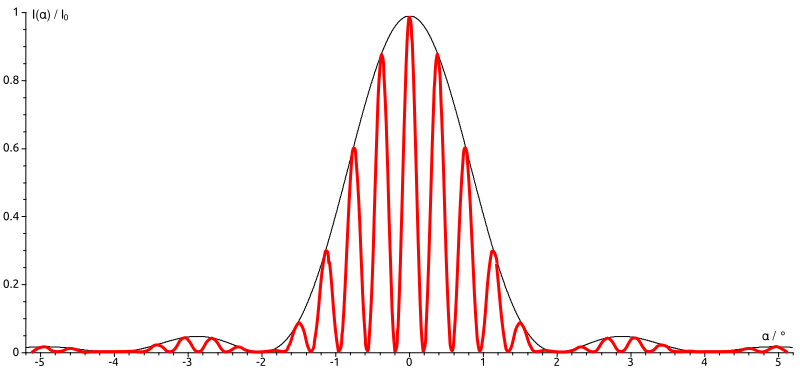
\includegraphics[width=0.4\textheight]{../figures/Slit_double.png}
  \caption{Intensitätsverteilung bei Beugung am Einzelspalt (schwarz) und Doppelspalt (rot). [By Klaus-Dieter Keller]}
\label{fig:slit}
\end{figure}


%This is the end

\clearpage
\newpage
\newpage

\section{Gaußsche Fehlerrechnung}\label{gausssche-fehlerrechnung}

\subsection{Berechnung der
Standardabweichung}\label{berechnung-der-standardabweichung}

Alle Messwerte sind als empirische Mittelwerte mit ihrer geschätzten
Standardabweichung des Mittelwertes angegeben. Diese unterschätzt die
wahre Standardabweichung, da die Wurzel aus der geschätzten Varianz
gezogen wird. Der arithmetische Mittelwert ist definiert als

\begin{align}
    \bar x = \frac{1}{n} \  \sum_{i=1}^n x_i \  .
    \label{equ:mean}
\end{align}

Die geschätzte Standardabweichung ist gegeben durch

\begin{align}
    s = \sqrt{\frac{1}{n-1} \sum_{i=1}^n (x_i - \bar x)^2}
    \label{equ:s}
\end{align}

mit der geschätzten Standardabweichung des Mittelwertes als

\begin{align}
    \Delta \bar x = \frac{s}{ \sqrt{n} }
    \label{equ:stdofmean}
\end{align}

\subsection{Gaußsche
Fehlerfortpflanzung}\label{gausssche-fehlerfortpflanzung}

Das Berechnen von Funktionen mit fehlerbehafteten Parametern erfolgt
mittels der Gauß'schen Fehlerfortpflanzung

\begin{align}
    \Delta f = \sqrt{ \sum_{i=1}^n \left( \frac{\diff f}{\diff y_i} \right)^2 (\Delta y_i)^2} \qquad \qquad \mathrm{mit} \quad f(y_1, \ldots , y_n)
    \label{equ:gauss}
\end{align}

\clearpage
\newpage
\section{Aufbau und Durchführung}
\subsection{Aufbau}
\label{sec:Aufbau}

Der Franck-Hertz-Versuch, Abbildung \ref{lel}, wird in einer Röhre durchgeführt, in der sich zwei Elektroden sowie ein Glühdraht befinden.
Der Glühdraht, auf dem eine konstante Heizspannung gegeben wird, dient durch den auftretenden glühelektrischen Effekt als Elektronenquelle.
Hierzu wird ein Metall mit einem hohen Schmelzpunkt, beispielsweise Wolfram, verwendet, so dass eine Elektronenwolke entsteht.
Diese Elektronen werden zu einer gitterförmigen Beschleunigungselektrode beschleunigt, welche sich in der Mitte der Röhre befindet.
Durch Wahl einer passenden Beschleunigungsspannung $U_B$ kann die Energiezufuhr der Elektronen gesteuert werden.
Am Ende des Gefäßes befindet sich zudem eine Auffängerelektrode, welche die Elektronen durch eine zwischen der Beschleunigungs- und Auffängerelektrode anliegenden Spannung $U_A$ abbremst.
Die Anzahl der auftreffenden Elektronen kann mithilfe eines Picoamperemeters anhand des Auffängerstroms $I_A$ bestimmt werden.
Dieses Messgerät verstärkt und wandelt den geringen Eingangsstrom um, so dass dieser als Spannung auf die Y-Achse eines XY-Schreibers gegeben werden kann.
Durch das zusätzliche Anlegen von $U_A$ oder $U_B$ am X-Eingang wird somit der Eingangsstrom in Abhängigkeit einer variablen Beschleunigungs- oder Bremsspannung graphisch dargestellt.
\\

Zudem ist in der evakuierten Röhre eine geringe Menge Quecksilber platziert, welches je nach gewählter Umgebungstemperatur $T$ einen variablen Dampfdruck $p_\text{sät}$ besitzt.
Die Temperatur wird mittels eines elektronischen Temperaturreglers geregelt und anhand eines zusätzlich angebrachten Thermometers kontrolliert.

\begin{figure}[H]
  \centering
  \includegraphics[height=6cm]{ressources/aufbau2.png}
  \caption{Aufbau des Franck-Hertz-Versuchs. \cite{skript}}
  \label{lel}
\end{figure}

\clearpage
\newpage
\section{Durchführung}
\label{sec:Durchführung}
Als Strahlungsquelle wird im folgenden Versuch ein Thallium-Isotop verwendet.

\subsection{Aufnahme der Charakteristik des Zählrohrs}
Der $\beta$-Strahler wird vor dem Geiger-Müller-Zählrohr positioniert, um die Charakteristik des Strahlers aufzunehmen. Dazu wird die Anzahl der eingehenden Teilchen in Abhängigkeit der angelegten Spannung $U$ gemessen. Im Bereich von $\SI{320}{\volt}$-$\SI{700}{\volt}$ wird im Abstand von $\SI{10}{\volt}$ die dazugehörige Teilchenzahl $\Delta N$ notiert.
Bei der Durchführung ist darauf zu achten, die Spannung von $\SI{720}{\volt}$ nicht zu überschreiten, da sonst durch Dauerentladungen das Zählrohr zerstört wird.

\subsection{Sichtbarmachung von Nachentladungen}
In diesem Teil soll die Nachentladung rein qualitativ gezeigt werden. Dafür wird der Abstand des $\beta$-Strahlers zum Zählrohr vergrößert, bis auf dem Oszilloskop kein weiterer Impuls des Strahlers mehr sichtbar ist. Das entstehende Bild soll einmal bei einer Spannung von $\SI{350}{\volt}$ untersucht werden, da in diesem Bereich Nachentladungen sehr unwahrscheinlich sind und einmal bei $\SI{700}{\volt}$.

\subsection{Oszillographische Messung der Totzeit}
Es wird die Strahlungsintensität erhöht indem der $\beta$-Strahler nah am Zählrohr positioniert wird. Auf dem Oszilloskop wird die Totzeit $T$ und die Erholungszeit $T_\textrm{E}$ grob abgeschätzt.


\subsection{ Bestimmung der Totzeit mit der Zwei-Quellen-Methode}
\label{sec:Totzeit}
Zuerst wird die erste Strahlungsquelle vor dem Zählrohr platziert und die Zählrate $N_1$ aufgenommen. Dann wird ein zweiter Strahler vor dem Zählrohr platziert und die Zählrate $N_\textrm{1+2}$ aufgenommen. Zuletzt wird die erste Quelle wieder entnommen um die Zählrate $N_2$ auf zu nehmen.\\
Aufgrund der Totzeit gilt
\begin{align}
  N_\textrm{1+2} < N_\textrm{1} + N_\textrm{2}\;.
  \label{eq:N1und2}
\end{align}
Auf Grundlage von Gleichung $\ref{eq:N}$ wird die Totzeit $T$ bestimmt durch
\begin{align}
  T \approx \frac{N_\textrm{1} + N_\textrm{2} - N_\textrm{1+2}}{2N_\textrm{1} N_\textrm{2}} \;.
  \label{eq:T}
\end{align}

\subsection{Messung der pro Teilchen vom Zählrohr freigesetzten Ladungsmenge }
Mit einem geeigneten Amperemeter wird der mittlere Zählrohrstrom
\begin{align}
  \bar{I} \coloneqq \frac{1}{\tau} \int_0^\tau \frac{U(t)}{R} dt
  \label{eq:Strom1}
\end{align}
wobei $\tau >> T$, gemessen.
Da die Anzahl der Teilchen $Z$ und das Zeitintervall $\Delta t$, in dem die Teilchenzahl bestimmt wird, bekannt ist, ergibt sich mit der Definition des Stroms
\begin{align}
  \bar{I} = \frac{\Delta Q}{\Delta t} Z\;.
  \label{eq:Strom2}
\end{align}
Auf Grund der Abhängigkeit der Ladungsmenge von der Zählrohrspannung, wird $\Delta Q$ während der Aufnahme der Charakteristik des Zählrohres notiert.

\clearpage
\newpage
\section{Auswertung}
\label{sec:Auswertung}

% % Examples
% \begin{equation}
%   U(t) = a \sin(b t + c) + d
% \end{equation}
%
% \begin{align}
%   a &= \input{build/a.tex} \\
%   b &= \input{build/b.tex} \\
%   c &= \input{build/c.tex} \\
%   d &= \input{build/d.tex} .
% \end{align}
% Die Messdaten und das Ergebnis des Fits sind in Abbildung~\ref{fig:plot} geplottet.
%
% %Tabelle mit Messdaten
% \begin{table}
%   \centering
%   \caption{Messdaten.}
%   \label{tab:data}
%   \sisetup{parse-numbers=false}
%   \begin{tabular}{
% % format 1.3 bedeutet eine Stelle vorm Komma, 3 danach
%     S[table-format=1.3]
%     S[table-format=-1.2]
%     @{${}\pm{}$}
%     S[table-format=1.2]
%     @{\hspace*{3em}\hspace*{\tabcolsep}}
%     S[table-format=1.3]
%     S[table-format=-1.2]
%     @{${}\pm{}$}
%     S[table-format=1.2]
%   }
%     \toprule
%     {$t \:/\: \si{\milli\second}$} & \multicolumn{2}{c}{$U \:/\: \si{\kilo\volt}$\hspace*{3em}} &
%     {$t \:/\: \si{\milli\second}$} & \multicolumn{2}{c}{$U \:/\: \si{\kilo\volt}$} \\
%     \midrule
%     1.7 & 10 \\
2.3 & 20 \\
3.5 & 30 \\
4.4 & 40 \\

%     \bottomrule
%   \end{tabular}
% \end{table}
%
% % Standard Plot
% \begin{figure}
%   \centering
%   \includegraphics{build/plot.pdf}
%   \caption{Messdaten und Fitergebnis.}
%   \label{fig:plot}
% \end{figure}
%
% 2x2 Plot
% \begin{figure*}
%     \centering
%     \begin{subfigure}[b]{0.475\textwidth}
%         \centering
%         \includegraphics[width=\textwidth]{Abbildungen/Schaltung1.pdf}
%         \caption[]%
%         {{\small Schaltung 1.}}
%         \label{fig:Schaltung1}
%     \end{subfigure}
%     \hfill
%     \begin{subfigure}[b]{0.475\textwidth}
%         \centering
%         \includegraphics[width=\textwidth]{Abbildungen/Schaltung2.pdf}
%         \caption[]%
%         {{\small Schaltung 2.}}
%         \label{fig:Schaltung2}
%     \end{subfigure}
%     \vskip\baselineskip
%     \begin{subfigure}[b]{0.475\textwidth}
%         \centering
%         \includegraphics[width=\textwidth]{Abbildungen/Schaltung4.pdf}    % Zahlen vertauscht ... -.-
%         \caption[]%
%         {{\small Schaltung 3.}}
%         \label{fig:Schaltung3}
%     \end{subfigure}
%     \quad
%     \begin{subfigure}[b]{0.475\textwidth}
%         \centering
%         \includegraphics[width=\textwidth]{Abbildungen/Schaltung3.pdf}
%         \caption[]%
%         {{\small Schaltung 4.}}
%         \label{fig:Schaltung4}
%     \end{subfigure}
%     \caption[]
%     {Ersatzschaltbilder der verschiedenen Teilaufgaben.}
%     \label{fig:Schaltungen}
% \end{figure*}

\clearpage
\newpage
\section{Diskussion}
\label{sec:Diskussion}
Die Messung der Schallgeschwindigkeit mittels Impuls-Echo-Verfahren liefert einen Wert von
\begin{align*}
  c_{\text{acryl,e}} &= \input{build/c_acryl_1.tex}.
\end{align*}
Daraus folgt eine Abweichung zum Literaturwert \cite{acryl},
\begin{align*}
  c_{\text{acryl,lit}} &= \input{build/v_lit.tex},
\end{align*}
von
\begin{align*}
  \increment c_{\text{acryl}} &= \input{build/v_rel_1.tex}.
\end{align*}
Bei der Durchschallungs-Methode ergibt sich für die Phasengeschwindigkeit in Acryl
\begin{align*}
  c_{\text{acryl,d}} &= \input{build/c_acryl_2.tex},
\end{align*}
die relative Abweichung zum Literaturwert beträgt hier
\begin{align*}
  \increment c_{\text{acryl,d}} &= \input{build/v_rel_2.tex}.
\end{align*}
Die dritte Bestimmung der Schallgeschwindigkeit erfolgte über die Steigung der Ausgleichsrechnung, hier ergab sich ein Wert von
\begin{align*}
  c_{\text{acryl, a}} &= \input{build/parameter_a.tex}
\end{align*}
mit einer relativen Abweichung von
\begin{align*}
  \increment c_{\text{acryl,a}} &= \input{build/v_rel_3.tex}.
\end{align*}
Die Impuse-Echo-Methode erweist sich dementsprechend als exakteste.\\
Die Anpassungsschicht wurde mittels y-Achsenabschnitt der Ausgleichsrechnung zu
\begin{align*}
  d &= \input{build/parameter_b.tex}.
\end{align*}
Dieser Wert scheint eine gute Beschreibung der Anpassungsschicht zu sein, da laut Literatur eine Dicke von durchschnittlich $\SI{0.5}{\milli\metre}$ bis zu $\SI{2.5}{\milli\metre}$ zu erwarten ist. \cite{anpassungsschicht}\\
Bei der Ausmessung der Plattendicken mittels Cepstrum und FFT konnte jeweils nur eine Länge
\begin{align*}
  s_\text{fft} &= \input{build/s_probe.tex}, \\
  s_\text{cep} &= \input{build/s_cep.tex},
\end{align*}
unbekannter Bedeutung bestimmt werden.
Vermutlich handelt es sich hierbei um die kombinierte Dicke beider Platten.\\
Die Untersuchung des Augenmodelles führte auf die Längen
\begin{align*}
  s_{1} &= \input{build/s_12.tex}, \\
  s_{2} &= \input{build/s_23.tex}, \\
  s_{3} &= \input{build/s_36.tex}, \\
\end{align*}
welche ungefähr die Größe skalierte Größe eines menschlichen Auges beschreiben.

\clearpage
\newpage

\printbibliography

\clearpage
\newpage
\begin{appendix}
\section{Messdaten}
\centering
\begin{figure}
\includepdf[width=0.9\textwidth, pages={2}]{ressources/messdaten.pdf}
\end{figure}
\newpage
\begin{figure}
\includepdf[width=0.9\textwidth, pages={1}]{ressources/messdaten.pdf}
\end{figure}

\end{appendix}


\end{document}


% % Examples
% \begin{equation}
%   U(t) = a \sin(b t + c) + d
% \end{equation}
%
% \begin{align}
%   a &= \input{a.tex} \\
%   b &= \input{b.tex} \\
%   c &= \input{c.tex} \\
%   d &= \input{d.tex} .
% \end{align}
% Die Messdaten und das Ergebnis des Fits sind in Abbildung~\ref{fig:plot} geplottet.
%
% %Tabelle mit Messdaten
% \begin{table}
%   \centering
%   \caption{Messdaten.}
%   \label{tab:data}
%   \sisetup{parse-numbers=false}
%   \begin{tabular}{
%     S[table-format=1.3]
%     S[table-format=-1.2]
%     @{${}\pm{}$}
%     S[table-format=1.2]
%     @{\hspace*{3em}\hspace*{\tabcolsep}}
%     S[table-format=1.3]
%     S[table-format=-1.2]
%     @{${}\pm{}$}
%     S[table-format=1.2]
%   }
%     \toprule
%     {$t \:/\: \si{\milli\second}$} & \multicolumn{2}{c}{$U \:/\: \si{\kilo\volt}$\hspace*{3em}} &
%     {$t \:/\: \si{\milli\second}$} & \multicolumn{2}{c}{$U \:/\: \si{\kilo\volt}$} \\
%     \midrule
%     1.7 & 10 \\
2.3 & 20 \\
3.5 & 30 \\
4.4 & 40 \\

%     \bottomrule
%   \end{tabular}
% \end{table}
%
% % Standard Plot
% \begin{figure}
%   \centering
%   \includegraphics{plot.pdf}
%   \caption{Messdaten und Fitergebnis.}
%   \label{fig:plot}
% \end{figure}
